\section{Evaluation}

\subsection{Microbenchmarks}
\label{q_microbenchmarks}

All queues are evaluated on a set of microbenchmarks to demonstrate their scalability and performance. The controlled nature of these microbenchmarks allow us to easily compare particular aspects of each algorithm, such as transactional overhead introduced by STO. All experiments are run on a 100GB DRAM machine with two 6-core Intel Xeon X5690 processors clocked at 3.47GHz. Hyperthreading is enabled in each processor, resulting in 24 available logical cores. The machine runs a 64-bit Linux 3.2.0 operating system, and all benchmarks and STO data structures are compiled with g++-5.3. In all graphs, we show the median of 5 consecutive runs with the minimum and maximum performance results represented as error bars.

\subsubsection{Parameters}

\begin{itemize}
\item Value Types: Each queue benchmark uses randomly chosen integers. This is because the benchmark tests do not manipulate the values they push/pop and the queue algorithms are agnostic to the actual values being placed in the queue.

\item Initial Queue Size: We run several tests with different initial fullness of the data structure. This affects how often the structure becomes empty, which can cause aborts and additional overhead (as described in the algorithms above). It also affects the number of cache lines accessed: a near-empty queue will never require iterating over values contained in more than one cache line.

\item Transaction Size: We modify the number of operations per transaction in different benchmarks. For some benchmarks, the number of operations in a transaction is set to 1 (i.e., the transactions are singleton transactions). This provides a more fair evaluation of transactional data structures against concurrent data structures: by keeping a transaction as short as possible, we minimize the performance hit from transactional overhead. In order to support multiple-operation transactions, STO adds overhead which includes support for multiple items in read/write sets, read-my-writes, and an increased number of aborts and retries. With single operation transactions, we observe an upper bound on the best performance our data structures can achieve.

\item Data Structure Opacity: If opacity is enabled, a transaction will abort immediately if any inconsistent state is detected. This requires keeping track of a global transaction ID (TID). This global TID must be accessed when a transaction commits and when items are added to the read set during a transaction's, making transactions overall more expensive. For our benchmarks, we consider only queues without opacity enabled (as to measure its maximum achievable performance).\lyt{do we need this?}
\end{itemize}

\subsubsection{Tests}
\begin{enumerate}
\item 2-Thread Push-Pop Test: This test has one thread that performs only pushes and another thread that performs only pops. Unless the queue is empty, the two threads should never be modifying the same part of the data structure, and will never conflict (abort rate should be near 0). We use this test to measure the speed of push/pops on the queue when contention is not an issue. We expect that our transactional queues should perform as well, if not better, than most of the high-concurrency queues: while their algorithms are optimized for multi-threaded access, our simpler implementation should be just as fast with low contention and low abort rates.

\item Multi-Thread Singletons Test: 
    In this test, a thread randomly selects an operation (push or pop) to perform within each transaction. This keeps the queue at approximately the same size as its initial size during the test. This test is run with different initial queue sizes and different numbers of threads, which each thread performing singleton transactions. This test allows us to benchmark performance under variable amounts of contention (by increasing the number of threads) and increased abort rates. We expect that our STO-Queue1/STO-Queue2 transactional queues will perform significantly worse once the number of threads is increased and our naive concurrency algorithms underperform concurrency algorithms optimized for contentious situations.
    
%\item Multi-Thread Random Multi-Operation Transactions Test: 
    %In this test, a thread randomly selects multiple operations (push or pop) to perform within each transaction. This keeps the queue at approximately the same size as its initial size during the test. This test is run with different initial queue sizes and different numbers of threads. This test is most useful to compare different transactional data structures.
    
\end{enumerate}

\subsection{Results and Discussion}

We describe the results of these benchmarks for different sets of queues. We first compare the STO-Queue1 and STO-Queue2, then a set of high-concurrency, non-transactional queues, and lastly different variants of the flat-combining queue (transactional and non-transactional). The latter two sets are measured along with our STO-Queue2 as a baseline reference.

We refer to the several variants of the flat combining queue that we benchmark as follows:
\begin{itemize}
    \item FCQueueNT: the non-transactional flat combining queue.
    \item STO-FCQueue: the fully-transactional flat-combining queue.
    \item WrappedFCQueueNT: the non-transactional flat combining queue that invokes STO \texttt{start\_transaction} and \texttt{commit\_transaction} calls, but does not do any of the transactional bookkeeping necessary to provide transactional guarantees.
\end{itemize}


\subsubsection{STO-Queue1 vs. STO-Queue2}

\floatstyle{plain} 
\restylefloat{figure}
\begin{figure}[ht!]
\caption{STO-Queue1 vs. STO-Queue2}
    \centering
    \begin{tabular}{|c|c|}
        \hline&\\
        Speed (ops/s) & Aborts (\% Transactions)\\
        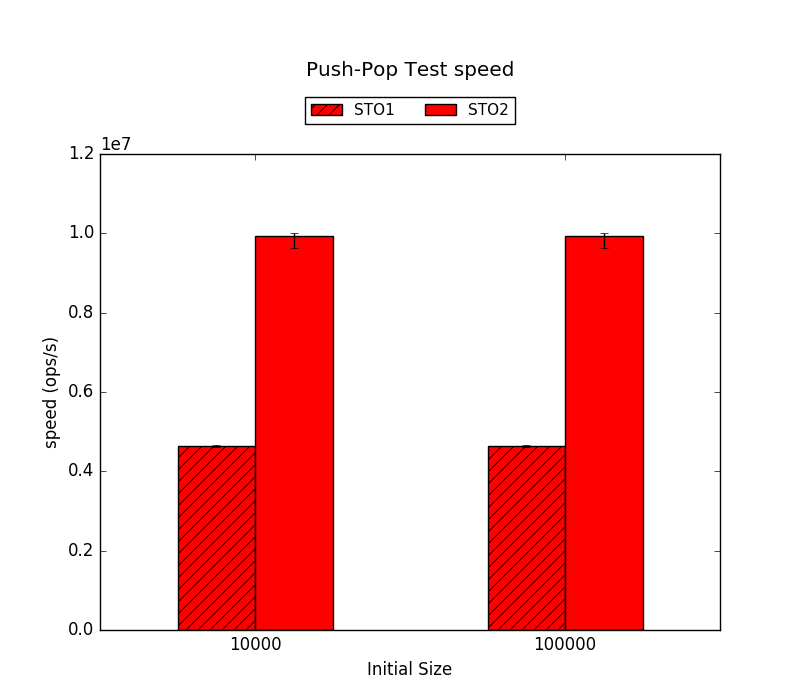
\includegraphics[height=2.25in]{fcqueues/stoQ:PushPopspeed.png} &
        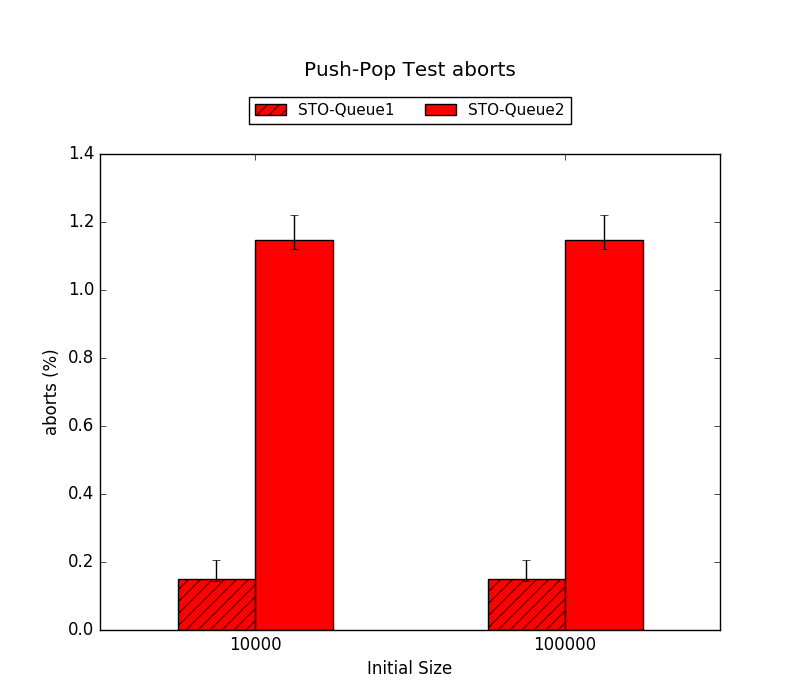
\includegraphics[height=2.25in]{fcqueues/stoQ:PushPopaborts.png}\\
        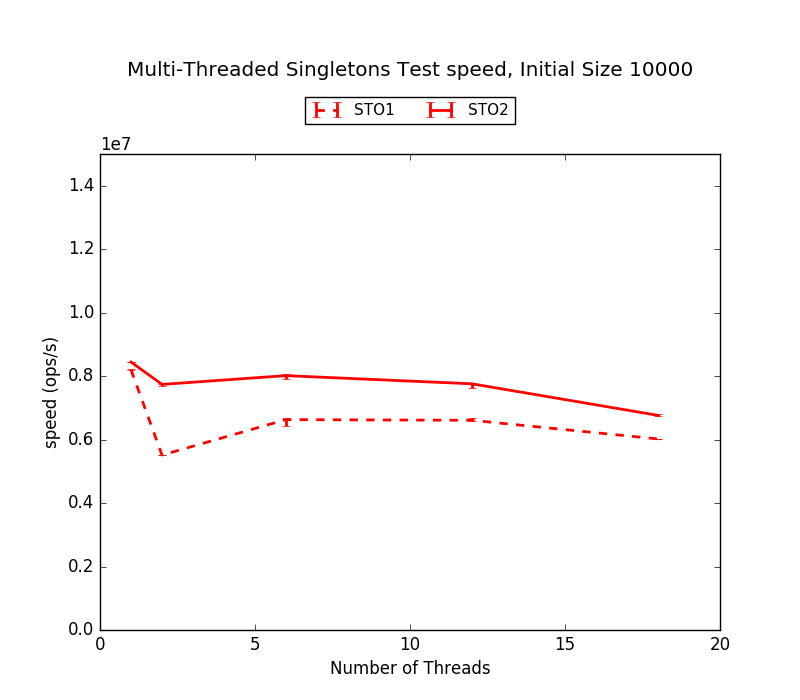
\includegraphics[height=2.25in]{fcqueues/stoQ:RandSingleOps10000speed.png} &
        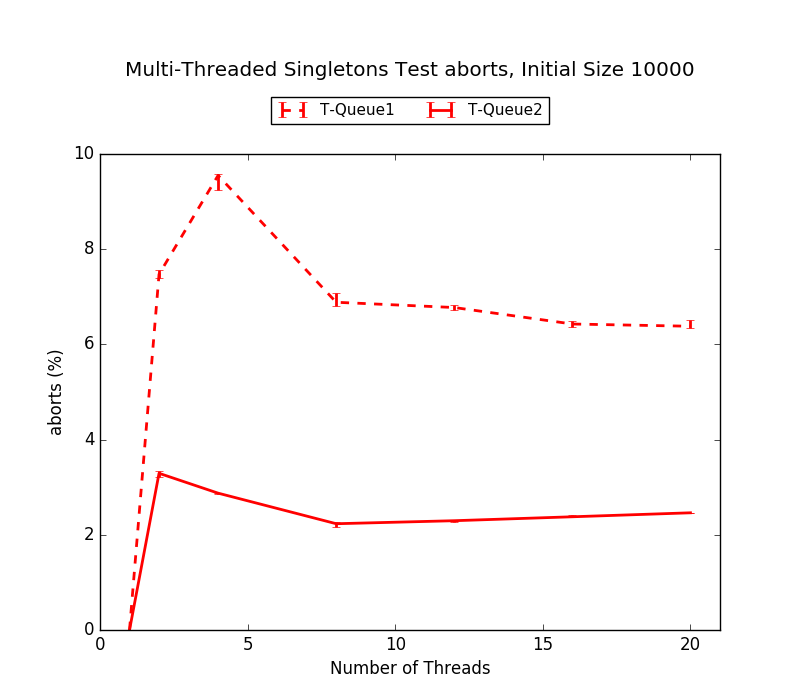
\includegraphics[height=2.25in]{fcqueues/stoQ:RandSingleOps10000aborts.png}\\
        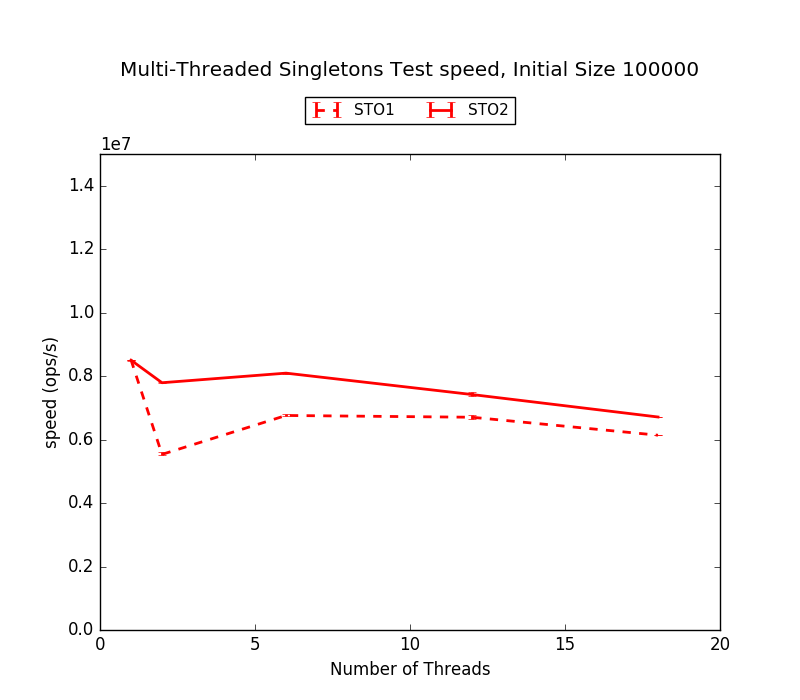
\includegraphics[height=2.25in]{fcqueues/stoQ:RandSingleOps100000speed.png} &
    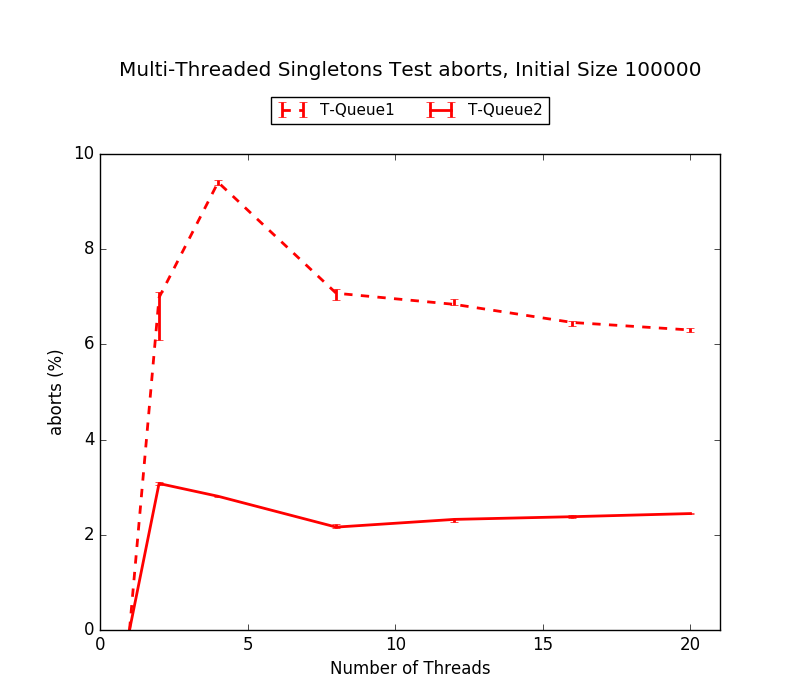
\includegraphics[height=2.25in]{fcqueues/stoQ:RandSingleOps100000aborts.png}\\
        \hline
    \end{tabular}
\label{fig:stoqueues}
\end{figure}

The performance results of STO-Queue1 and STO-Queue2 (Figure~\ref{fig:stoqueues}) can be compared to measure the effectiveness of a pessimistic approach to the pop operation. We use the better performing queue, the STO-Queue2, as the baseline reference in all future benchmarks.

\subsubsection{Concurrent, Non-transactional Queues}

We benchmark a set of the best-performing high-concurrency queue algorithms against the better performing STO queue implementation, the STO-Queue2. This helps determine which high-concurrency algorithm would be best suited to integration with STO. We look for both the most scalable and the highest-performing queue.
 
 Our implementation of the flat combining queue modifies the implementation of the flat combining queue from the authors of the flat combining paper\cite{flatcombining}. Our implementation of the other high-concurrency queues are taken from the Concurrent Data Structures (CDS) library implementations online\cite{libcds}. The performance of these implementations on our tests the performance results given in the papers that originally proposed the algorithms.\lyt{CHECK}

\floatstyle{boxed} 
\restylefloat{figure}
\begin{figure}[h!]
\centering
    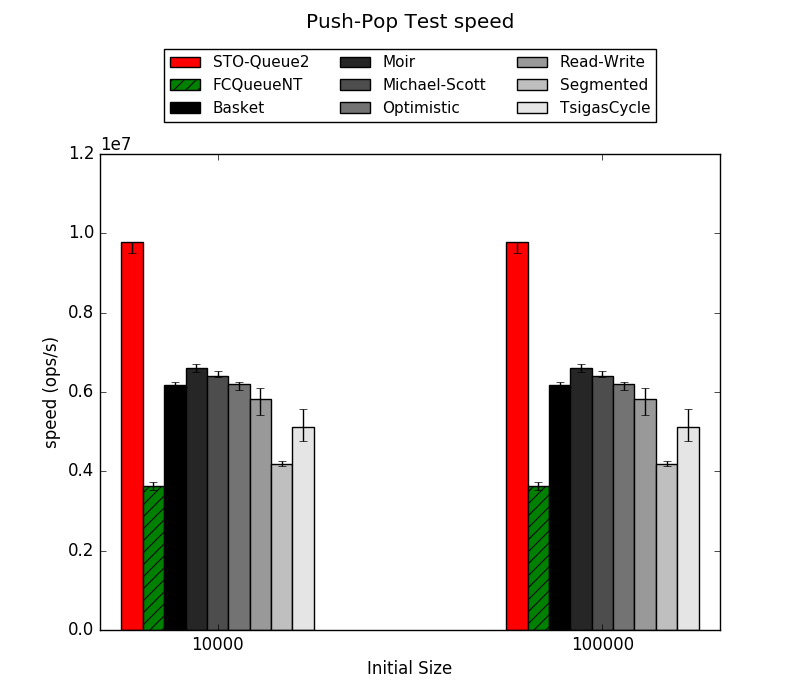
\includegraphics[height=3in]{concurrent/Q:PushPopspeed.png}\\
    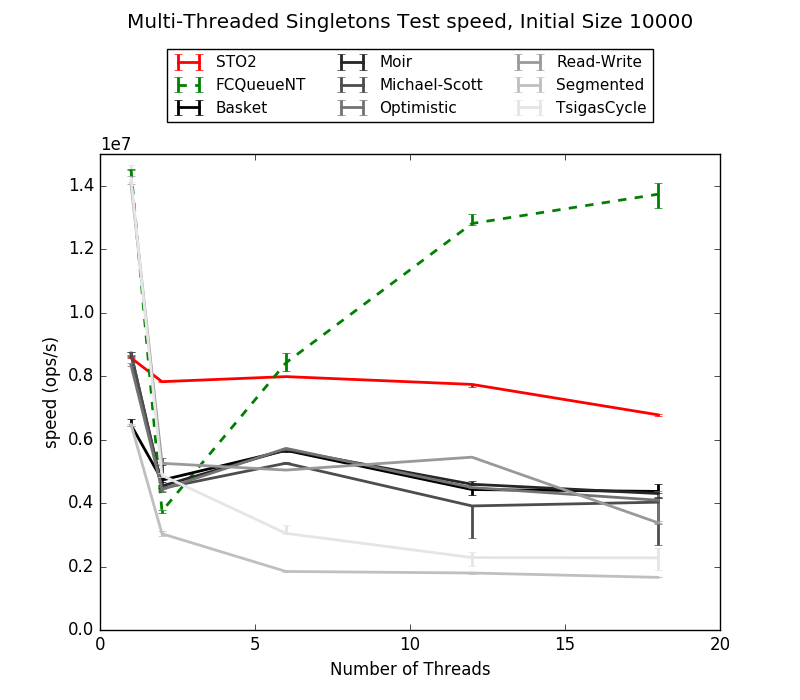
\includegraphics[height=3in]{concurrent/Q:RandSingleOps10000speed.png}
    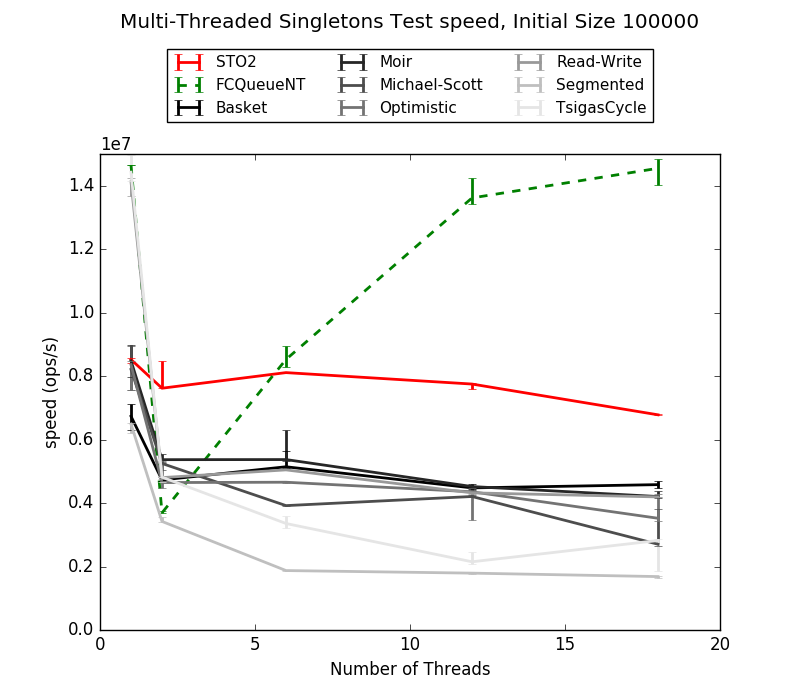
\includegraphics[height=3in]{concurrent/Q:RandSingleOps100000speed.png}
\caption{Performance of Various Concurrent Queues}
\label{fig:concurrent_queues}
\end{figure}

Out of the concurrent data structures tested, the Moir queue\cite{queue2} consistently performs best on the 2-Thread Push-Pop Test. On the Multi-Thread Singletons Test, the flat combining queue achieves performance over 2.5$\times$ greater than any other concurrent, non-transactional queue as the number of threads increases above 2.

The STO-Queue2 outperforms all queues on the 2-thread Push-Pop test. This test incurs the least contention and transactional overhead to track simply how fast the data structure can handle pushes and pops. It is unsurprising that, on this test, a simple synchronization strategy, such as that used in the STO queues, outperforms the majority of high-concurrency algorithms which are optimized for scalability. The Multi-Thread Singletons Test demonstrate that as contention and transactional overhead (abort rate) increases, the flat combining queue reaches performance approximately 1.75$\times$ greater than that of the STO queues. In addition, the flat combinig queue is the only queue that scales. All the other high-concurrency algorithms perform worse than our STO-Queue2 regardless of number of threads accessing the queue or initial queue size.
By benchmarking transactional queues with naive concurrency algorithms (STO-Queue1 and STO-Queue2) against various high-concurrency algorithms, we demonstrate that a simple implementation of a naive algorithm can consistently outperform more complex concurrent queue implementations even given the additional STO overhead. This indicates that the overhead added from STO does not cripple performance if used carefully---our transactional data structures can compete with several high-concurrency, non-transactional data structures. However, we see by comparing to the non-transactional flat combining queue that our algorithms are certainly not optimal for performance in a non-transactional setting.

Given these results, as well as the algorithmic benefits of the flat combining technique described in Section~\ref{fcqueuent}, we focus our work on the flat combining queue.


\subsubsection{WrappedFCQueueNT Performance}
The relative performance of the WrappedFCQueueNT to the FCQueueNT indicates how much of the overhead added by the STO system is unavoidable (without modifications to STO itself). The STO wrapper calls (\texttt{start\_transaction} and \texttt{commit\_transaction}) allow a thread to mark which operations should occur together in the same transaction. After invoking the \texttt{start\_transaction} call, the thread can collect items in its read- and write-sets; when \texttt{commit\_transaction} is invoked, the commit procedure is run (validation and installation of items in the read- and write-sets). The WrappedFCQueueNT adds no items to the read- and write-sets after invoking \texttt{start\_transaction}, and thus incurs the minimum amount of overhead necessary to use STO:\ the commit procedure has zero items to validate or install. The WrappedFCQueueNT therefore represents the upper bound on what performance we can expect from a fully transactional flat combining queue, the STO-FCQueue. 
Results are shown in Figure~\ref{fig:ntqueues}. 

When run with fewer than 10 threads, the STO wrapper calls can lead to performance 40\% worse than the vanilla non-transactional flat combining queue. However, once contention increases and becomes the bottleneck, the difference in performance becomes negligible. The WrappedFCQueueNT scales nearly equally as well as the FCQueueNT, particularly as the initial size of the queue increases. This comparison of the WrappedFCQueueNT and the FCQueueNT demonstrates that STO introduces negligible necessary overhead.  Even with the wrapper calls, our results indicate it can still be possible to achieve performance up to approximately 1.75$\times$ greater than that of our original STO-Queue1 and STO-Queue2 as the number of threads increases.

\begin{figure}[h!]
    \centering
    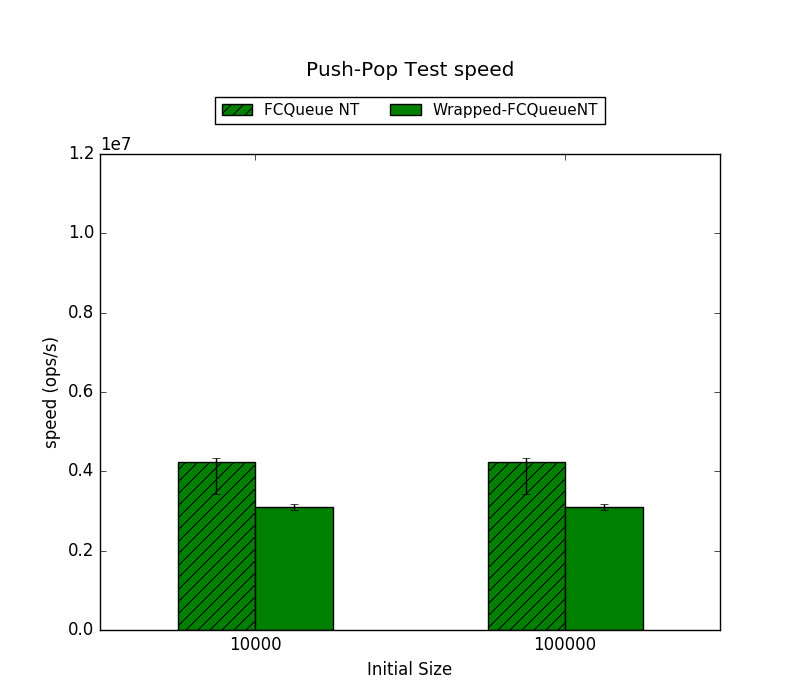
\includegraphics[height=3in]{fcqueues/ntQ:PushPopspeed.png}
    \\
    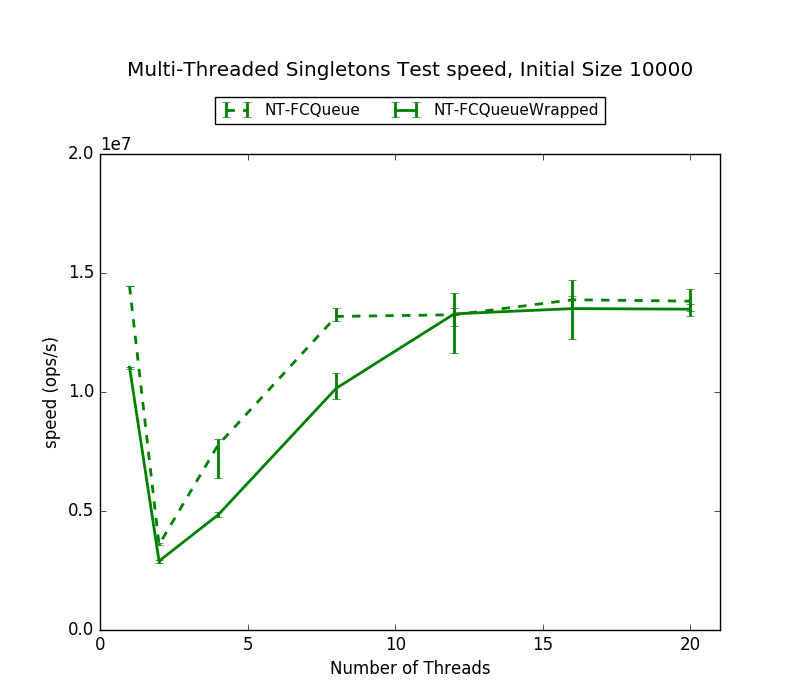
\includegraphics[height=3in]{fcqueues/ntQ:RandSingleOps10000speed.png}
    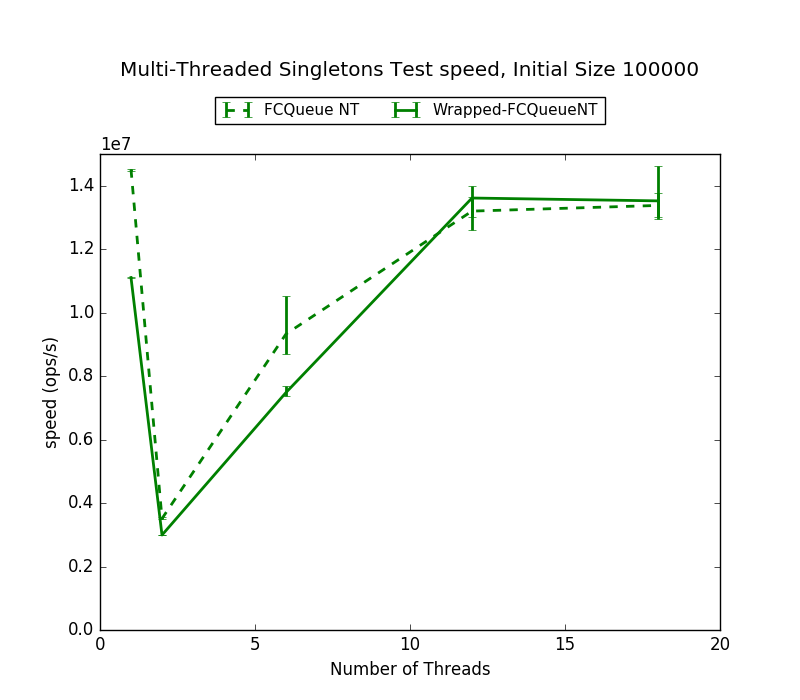
\includegraphics[height=3in]{fcqueues/ntQ:RandSingleOps100000speed.png}
\caption{WrappedFCQueueNT vs. FCQueueNT}
\label{fig:ntqueues}
\end{figure}

\subsubsection{STO-FCQueue Performance}
We compare the STO-FCQueue against the WrappedFCQueueNT and the STO-Queue2 to measure how the flat combining transactional approach described in Section~\ref{fcqueuet} performs.
Results are shown in Figure~\ref{fig:tfcqueues}.

\floatstyle{plain} 
\restylefloat{figure}
\begin{figure}[ht!]
\caption{STO-FCQueue Performance}
    \centering
    \begin{tabular}{|c|c|}
        \hline&\\
        Speed (ops/s) & Aborts (\% Transactions)\\
        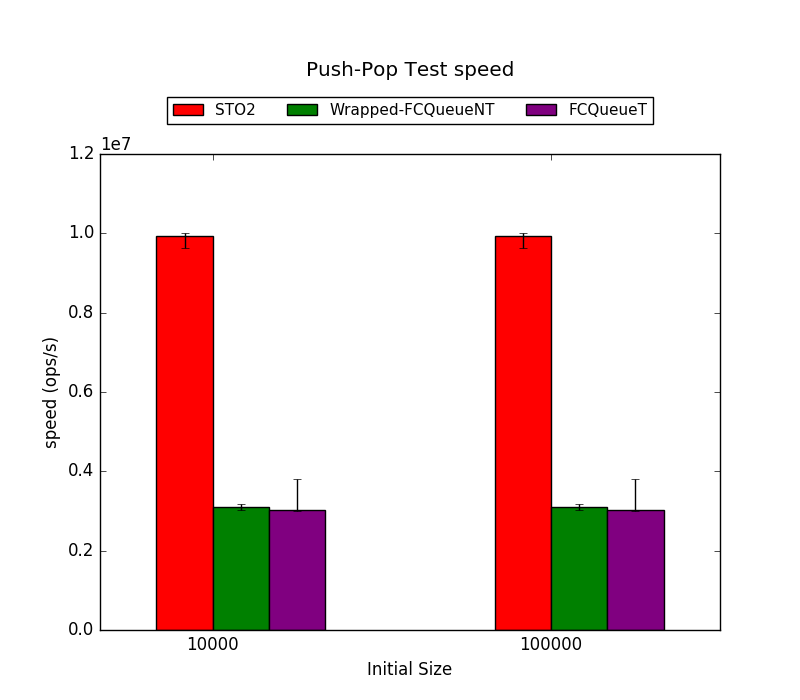
\includegraphics[height=2.25in]{fcqueues/tQ:PushPopspeed.png} &
        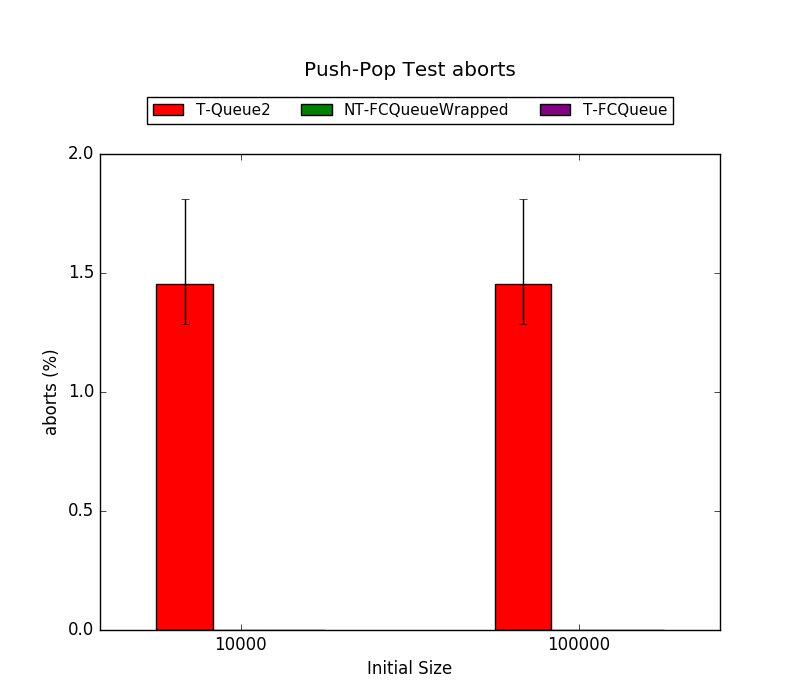
\includegraphics[height=2.25in]{fcqueues/tQ:PushPopaborts.png}\\
        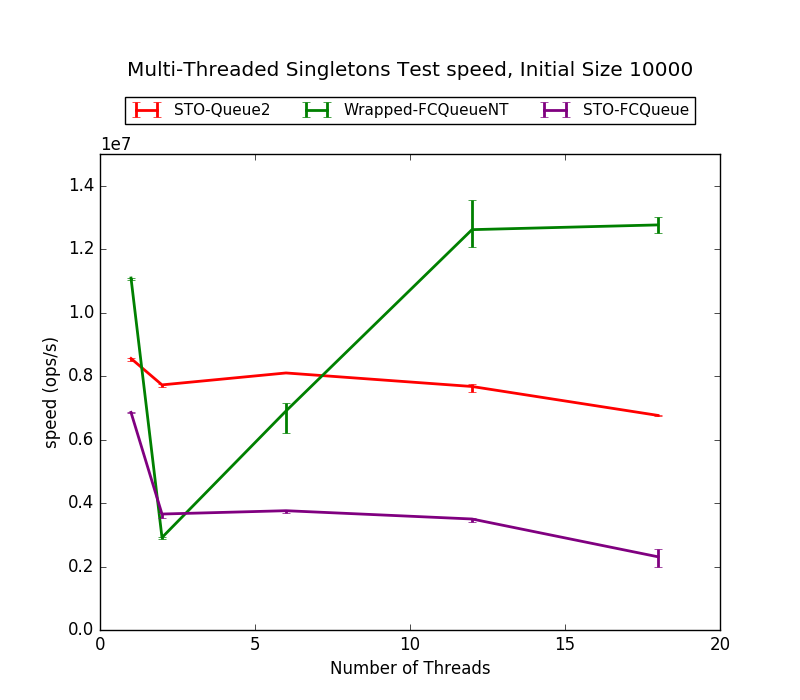
\includegraphics[height=2.25in]{fcqueues/tQ:RandSingleOps10000speed.png} &
        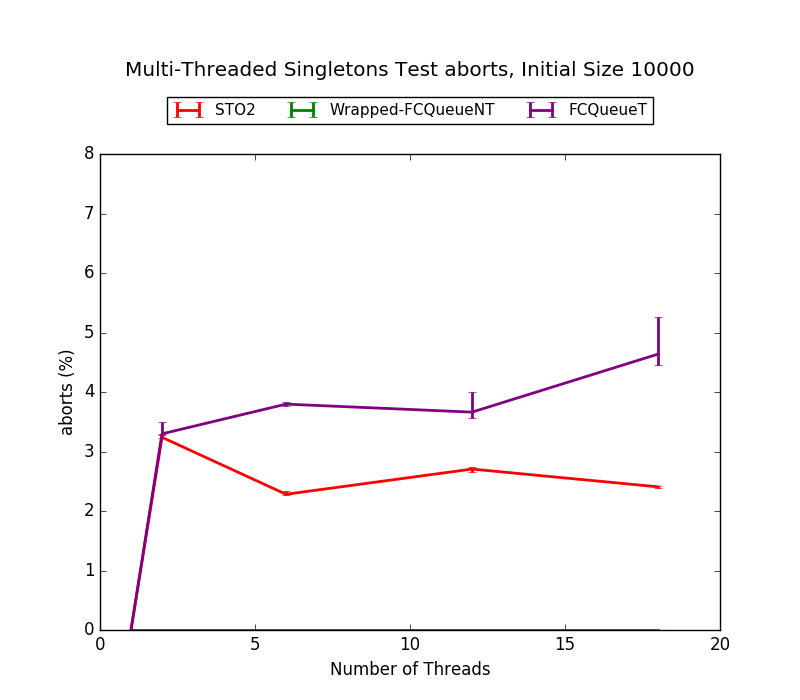
\includegraphics[height=2.25in]{fcqueues/tQ:RandSingleOps10000aborts.png}\\
        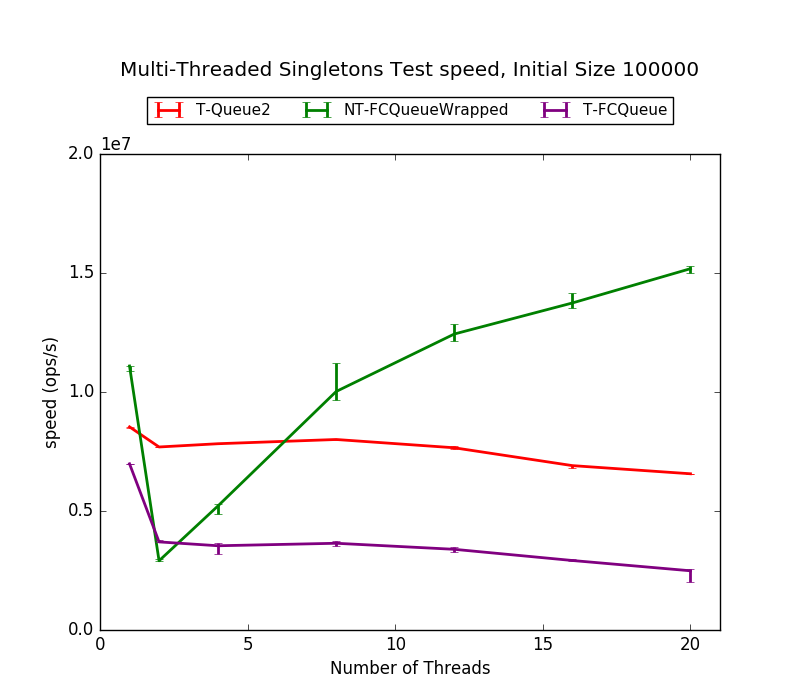
\includegraphics[height=2.25in]{fcqueues/tQ:RandSingleOps100000speed.png} &
    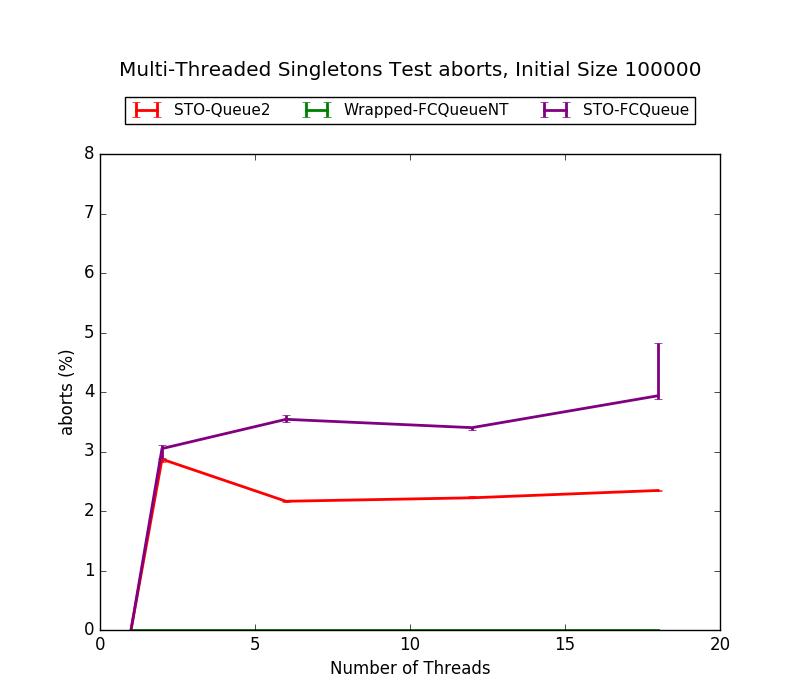
\includegraphics[height=2.25in]{fcqueues/tQ:RandSingleOps100000aborts.png}\\
        \hline
    \end{tabular}
\label{fig:tfcqueues}
\end{figure}

In the Push-Pop Test, the STO-Queue2 outperforms both flat combining variants, an unsurprising result given our results from the concurrent queues benchmark in Figure~\ref{fig:ntqueues}. We also note that only the STO-Queue2 experiences aborts (at approximately 1.2\% abort rates). We hypothesize this is due to a ``no-starvation'' aspect of the flat combining algorithm: the STO-Queue2's pop or push operations acquire a global queue lock. This means that the push-only or pop-only thread may continuously succeed in acquiring the lock, leading to a large sequence of pops or pushes. This can lead to the queue reaching an empty state more often, which is the only state that can cause commit-time checks to fail and the transaction to abort. The flat combining algorithm, however, applies the operations of both requesting threads during one combiner pass. Since one thread only pushes and the other only pops, no thread aborts due to seeing a marked pop, and the queue rarely reaches an empty state since both one push and one pop are applied during each pass.

The Multi-Threaded Singletons Test shows the STO-Queue2 performing approximately 2$\times$ better than the STO-FCQueue, regardless of initial queue size. Both queues do not scale, and the performance ratio remains constant regardless of the number of threads. The STO-FCQueue also experiences abort rates 1.5-2$\times$ of that of the STO-Queue2 as the number of threads increase.
Analysis with the \texttt{perf} tool indicates that the majority of the overhead is incurred from spinning on the flat combining lock (acquired by the combiner thread) or waiting for a flat combining call to complete. In addition, the number of cache misses is nearly 7$\times$ greater. We see these results because of two reasons:
\begin{enumerate}
\item \emph{Higher Quantity}: A thread must make multiple flat combining calls to perform a pop within a transaction (recall that a push only requires one flat combining call) 
\item \emph{Higher Complexity}: each flat combining call requires executing instructions, which makes each operation request more expensive.
\end{enumerate}

We conclude that the flat combining technique, while perhaps near-optimal for a highly-concurrent data structure, is no better in a transactional setting than a naive synchronization technique such as that used in the STO-Queue1 and STO-Queue2. This is because the flat combining algorithm must track the transaction state (e.g., going to perform two pops, one of which observes an empty queue) in order to provide transactional guarantees. In the next chapter, we formalize this argument using a commutativity discussion and claim that the higher quantity of more complex flat combining calls is necessary for flat combining to be used in a transactional setting: the flat combining technique depends on operation commutativity present in only a non-transactional setting to achieve its high performance. 
